\chapter{测试A}
\renewcommand\theequation{2-\arabic{equation}}
\blindtext
\section{我做的1个事}
\blindtext\cite{knuth1986the}\cite{lamport1989latex:}
\section{我又做的1个事}

1. 按照自用的课堂报告word模板的格式编写了这份LaTeX模板,封面的样式基础是材料学院提供的实习报告模板。本模板并非官方认证,亦存在着不少缺陷,请按照任课老师的具体要求完成作业,若因格式问题造成不必要损失的,恕不负责。

2. 模板的样式基准为article类型,标题分为三级,格式均不作任何改动。需要用到此模板时将cls文件放在需要编译的tex文件的目录下即可,需要插入图片时请将文件夹放在同一目录下并命名为pics。

3. 标题页仍计入页码数,请使用titlepage环境去除

4. 设置了序号、人名+时间、上角标序号三种引用类型,请根据需要在cls文件里进行调整。为保持前后文格式一致,未设置局部格式调整的参数

5. 图片应放置在pics文件夹中,标题图命名为title,矢量图推荐使用.pdf/.eps格式,像素图推荐使用.bmp/.jpg/.bmp格式

6. 默认引用格式为蓝色无框数字,参考文献与附录将不计入引用,不出现在目录中,可在编写document时酌情对目录进行修改。

7. 汉字默认字体为宋体,加粗为黑体,斜体为楷书。拉丁字母的默认字体为Times New Roman。

8. 作者使用环境为MikTex 2.9,利用xeTex+makeindex+bibtex编译
9. 若不新定义命令或改动了命令的输入参数,不会专门发布新的版本,最新改动以代码行贴出的cls文件为准。



\subsection{两个小标题q}

\begin{equation}
\ddot{d}=\frac{Q_{p}g}{\beta}-g=\frac{0.0034ge^{\frac{-y}{22000}} \dot{y}^{2}}{2\beta}-g \label{4}
\end{equation}

\subsection{两个小标题p}

\begin{equation}
\ddot{d}=\frac{Q_{p}g}{\beta}-g=\frac{0.0034ge^{\frac{-y}{22000}} \dot{y}^{2}}{2\beta}-g \label{4}
\end{equation}

\section{还是我做的1个事}

\begin{equation}
\ddot{d}=\frac{Q_{p}g}{\beta}-g=\frac{0.0034ge^{\frac{-y}{22000}} \dot{y}^{2}}{2\beta}-g \label{4}
\end{equation}

\begin{figure}[ht]
    \centering
    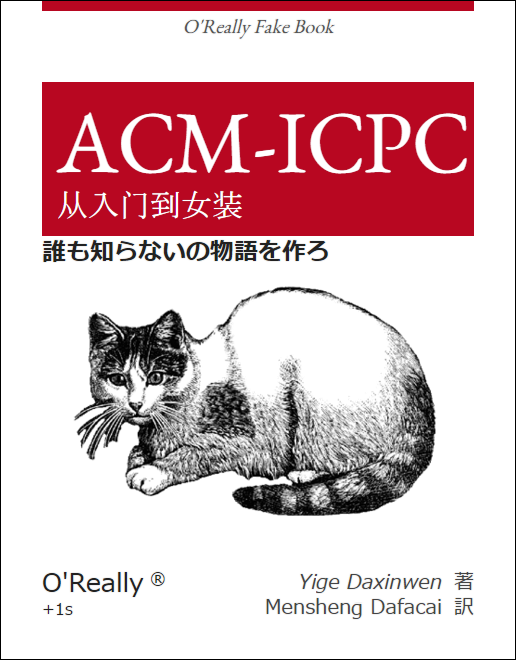
\includegraphics[scale=0.6]{figures/figure1.png}
    \caption{
        这里是个普通的标题
    }
    \label{fig:example}
\end{figure}
\endinput